\chapter{SÉMANTIQUE}
\label{chapter-11}
\markright{Sémantique}
\origpage{318}{304}
\begin{keybox}[Plan du chapitre]
\small\setstretch{1.01}
\setlist{topsep=.12em,itemsep=.12em,parsep=0pt}
\renewcommand{\thempfootnote}{校\arabic{editorialnote}}
\textbf{I.\quad MICHEL BRÉAL, LE FONDATEUR D’UNE NOUVELLE SCIENCE}
\begin{enumerate}[label=\arabic*.]
\item L’\textit{Essai de sémantique}
\item Le rejet de l’organicisme
\item L’inspirateur de Saussure
\end{enumerate}
\textbf{II.\quad LOUIS HJELMSLEV : LA SÉMANTIQUE STRUCTURALISTE}
\begin{enumerate}[label=\arabic*.]
\item La connotation et dénotation
\begin{enumerate}[label=\textcircled{\scriptsize\arabic*}]
\item Chez Port Royal : les idées accessoires
\item Chez Stuart Mill : la théorie de la référence directe
\item Chez Roland Barthes : la voie d’accès à la polysémie
\item Chez Hjelmslev : langages de connotation
\end{enumerate}
\item La glossématique
\begin{enumerate}[label=\textcircled{\scriptsize\arabic*}]
\item La notion de strata
\item Les formes de contenu
\item Les formes d’expression
\end{enumerate}
\end{enumerate}
\textbf{III.\quad BERNARD POTTIER : LA SÉMANTIQUE COMPONENTIELLE}
\begin{enumerate}[label=\arabic*.]
\item Les concepts et méthodes de l’analyse sémique
\begin{enumerate}[label=\textcircled{\scriptsize\arabic*}]
\item Sème, sémème, archisémème
\item L’exemple des noms de sièges
\item Archisémème, archilexème, hyperonyme
\end{enumerate}
\item Typologie des sèmes
\begin{enumerate}[label=\textcircled{\scriptsize\arabic*}]
\item Sèmes dénotatifs et sèmes connotatifs
\item Sèmes spécifiques et sèmes génériques
\end{enumerate}
\item Classement des sèmes
\begin{enumerate}[label=\textcircled{\scriptsize\arabic*}]
\item L’archisémème
\item Le sémantème
\item Le classème
\item Le virtuème
\item Le noème
\end{enumerate}
\end{enumerate}
\tcbbreak
\origpage{319}{305}
\textbf{IV.\quad JULIEN GREIMAS : LA SÉMANTIQUE TEXTUELLE}
\begin{enumerate}[label=\arabic*.]
\item Le modèle actantiel
\begin{enumerate}[label=\textcircled{\scriptsize\arabic*}]
\item Les six actants
\item Les trois axes
\end{enumerate}
\item L’isotopie
\begin{enumerate}[label=\textcircled{\scriptsize\arabic*}]
\item La notion de molécule sémique
\item Exemples en poésie
\end{enumerate}
\item Le carré sémiotique
\begin{enumerate}[label=\textcircled{\scriptsize\arabic*}]
\item Présentation
\item Éléments constitutifs\par 1. Les termes\par 2. Le métatermes\ednote{章首提纲 Le métatermes 应为 Les métatermes；正文对应小标题已用复数 Les。}
\item Les relations de contrariété et de contradiction
\item Application
\item Niveaux d’analyse
\end{enumerate}
\end{enumerate}
\textbf{V.\quad FRANÇOIS RASTIER : LA SÉMANTIQUE INTERPRÉTATIVE}
\begin{enumerate}[label=\arabic*.]
\item Les trois classes sémantiques
\begin{enumerate}[label=\textcircled{\scriptsize\arabic*}]
\item La dimension
\item Le domaine
\item Le taxème
\item Application
\end{enumerate}
\item Typologie sémique
\begin{enumerate}[label=\textcircled{\scriptsize\arabic*}]
\item Sèmes génériques et sèmes spécifiques
\item Sèmes inhérents et sèmes afférents
\item Application
\item Sèmes actualisés et sèmes virtualisés
\end{enumerate}
\item L’isotopie
\begin{enumerate}[label=\textcircled{\scriptsize\arabic*}]
\item Les isotopies génériques
\item Les isotopies spécifiques
\item Connexions métaphoriques et allotopie
\item La notion de poly-isotopie
\end{enumerate}
\end{enumerate}
\textbf{Exercices}\par\textbf{Pour aller plus loin}\par\textbf{Glossaire}
\end{keybox}

\origpage{320}{306}
\begin{keybox}[Introduction]
\renewcommand{\thempfootnote}{校\arabic{editorialnote}}
On attribue à Michel Bréal la paternité de la nouvelle « science des significations », qu’il a baptisée du nom de sémantique dans un article de 1883 (\textit{Les lois intellectuelles du langage}) puis présentée dans son \textit{Essai de sémantique} paru en 1897. Dire que la sémantique est la science des signification\ednote{原文 des signification 的数配合有误，应为 des significations。} implique de définir d’abord ce que l’on entend par signification, et cette tâche n’est pas aisée. Et une fois cette difficulté surmontée, une autre se présente à nous : la dissociation, fréquente dans les théories sémantiques, des concepts de sens et de signification. Cette seconde difficulté est aggravée par le fait qu’il n’y a pas de consensus figé dans le marbre, et que ces deux termes recouvrent des définitions différentes selon les écoles linguistiques. Cette distinction entre sens et signification apparaît pour la première fois dans la première édition de l’\textit{Encyclopédie} de Diderot et d’Alembert, en 1751.\ednote{1751 为《百科全书》第一卷刊年，不足以证明后文所引 « sens » 条目亦于该年刊行；且“首次区分”须另有历史文献依据。条目卷次、作者归属及刊年尚待核实，暂不据本句断言为首创。} Le grammairien et philosophe César Chesneau Dumarsais (1676-1756), rédacteur de l’article intitulé « sens » dans l’\textit{Encyclopédie des Lumières}, revient sur le « vague » qui entoure ces deux termes :

Ce mot [sens] est souvent synonyme de signification \& d’acception ; quand on n’a qu’à indiquer d’une manière vague et indéfinie la représentation dont les mots sont chargés, on peut se servir indifféremment de l’un ou de l’autre de ces trois termes. Mais il y a bien des circonstances où le choix n’est pas indifférent, parce qu’ils sont distingués l’un de l’autre par des idées accessoires qu’il ne faut pas confondre ».

Dumarsais va donc distinguer, afin de ne pas les confondre :
\begin{itemize}
\item la signification, le contenu d’un mot isolé : « chaque mot a d’abord une signification primitive et fondamentale qui doit être le principal objet à déterminer dans un dictionnaire, ainsi que dans la traduction littérale d’une langue en une autre »
\item le sens, contenu d’un mot dans le contexte d’une expression ou phrase : « quelquefois le mot est pris avec abstraction de l’objet qu’il représente [...] pour être rapporté à la classe de mots à laquelle il appartient. [...] Le sens est une autre signification différente de la primitive qui est moins indiquée par le mot même que par sa combinaison avec les autres qui constituent la phrase ».
\end{itemize}
Dans cette optique, on peut considérer que l’énoncé : « Donne-le moi »\ednote{规范拼写须以连字符连接肯定命令式后的两个代词，即 Donne-le-moi。此处按底本保留空格。} a toujours la même signification, à savoir une injonction adressée par un locuteur à un interlocuteur de lui donner quelque chose. Mais son sens variera pour chaque énoncé, selon le lieu, le temps, l’interlocuteur, c’est-à-dire le contexte d’énonciation. Ces précisions faites, nous pouvons commencer notre nouveau chapitre.
\end{keybox}

\Needspace{7\baselineskip}
\origpage{321}{307}
\section[MICHEL BRÉAL, LE FONDATEUR D’UNE NOUVELLE SCIENCE]{MICHEL BRÉAL, LE FONDATEUR\\D’UNE NOUVELLE SCIENCE}
\markright{Michel Bréal}
Entré en 1852 à l’École normale supérieure de Paris, \textbf{Michel Bréal} a étudié le sanskrit en 1857 à Berlin auprès du grammairien comparatiste \textbf{Franz Bopp}, dont il a traduit la volumineuse \textit{Grammaire comparée des langues indo-européennes}. Il est devenu ensuite professeur de grammaire comparée à l’École pratique des hautes études, puis au Collège de France, de 1866 à 1905. Dans les leçons d’ouverture de son cours au Collège de France, Bréal a d’emblée précisé :
\begin{quote}\small\itshape
L’histoire des formes du langage n’est que la moitié de la grammaire comparative et que cette étude purement extérieure des mots doit toujours être éclairée et contrôlée par l’examen de la signification.
\end{quote}
Dans les années 1880, l’influence de Bréal était considérable. Saussure, qui se trouvait à Paris à cette époque, est devenu son disciple. Nous verrons un peu plus bas l’influence du maître sur son disciple.

\subsection{L’\textit{Essai de sémantique}}
Paru en 1897 avec le sous-titre « science des significations », l’\textit{Essai de sémantique} aurait pu avoir pour sous-titre « science des signes linguistiques », car la sémantique de Bréal est en fait une linguistique générale. L’année de sa publication, le philologue et médiéviste \textbf{Antoine Thomas (1857-1935)} a écrit à propos du livre de Bréal :
\begin{quote}\small\itshape
Telle que la pratique M. Bréal, la sémantique nous apparaît moins comme une science distincte que comme une certaine façon d’entendre et d’étendre la linguistique. C’est une sorte de linguistique supérieure, un extrait, une quintessence de linguistique.
\end{quote}
Son \textit{Essai de sémantique} a été précédé par plusieurs essais, comme \textit{L’Histoire des mots} (1887) ou \textit{Le Langage et les nationalités} (1891), qui offrent un exposé condensé de sa sémantique qui ont été en grande partie intégrés dans son ouvrage de 1897. Mais c’est en 1883, dans \textit{Les Lois intellectuelles du langage. Fragment de sémantique} (1883), qu’il baptise cette science qu’il est en train de fonder\origfoot{1}{Quelques années plus tard, Saussure fera de même avec la sémiologie.} :
\begin{quote}\small\itshape
Comme cette étude, aussi bien que la phonétique ou la morphologie, mérite d’avoir son nom, nous l’appellerons la sémantique, c’est-à-dire la science des significations.
\end{quote}
Le terme de « sémantique », quant à lui, est un peu plus ancien et apparaît dès 1879 dans une lettre de Bréal adressée au linguiste et orientaliste italien \textbf{Angelo de Gubernatis} (1840-1913) :
\begin{quote}\small\itshape
Je prépare aussi un livre sur les lois intellectuelles du langage, auquel je travaille depuis des années : c’est ce qu’on peut appeler la sémantique. Vous en avez entendu un spécimen à mon Cours.
\end{quote}

\Needspace{7\baselineskip}
\origpage{322}{308}
\subsection{Le rejet de l’organicisme}
Nous avons vu dans le chapitre 5 le naturaliste \textbf{August Schleicher} assimiler la langue à un organisme soumis aux lois de l’évolution et bannir de la linguistique l’esprit et la volonté. Bréal s’est opposé à cela et été l’ennemi implacable\ednote{原文 et été 缺少助动词，依句法应为 et a été。} de l’anthropologie biologique française, surtout en ce qui concerne les théories de l’évolution linguistique inspirées de Schleicher. En particulier, il reproche au comparatisme de se concentrer seulement sur la face phonique des langues, et de réduire ainsi la linguistique à une branche de la physiologie.
\begin{quote}\small\itshape
Dire que le langage est un organisme, c’est obscurcir les choses et jeter dans les esprits une semence d’erreur [...] Dire que les mots naissent, vivent entre eux et meurent, cela est, n’est-il point vrai, pure métaphore ? Parler de la vie du langage, appeler les langues des organismes vivants, c’est user de figures qui nous transporteraient en plein rêve [...]
\end{quote}
Remettant aussi en cause l’organicisme de son ancien professeur Franz Bopp, Bréal a réaffirmé l’importance de l’esprit, de la volonté et a déplacé le centre de gravité de la réflexion linguistique vers le lien entre le langage et la pensée. Ce faisant, il ne prétendait pas rejeter les phénomènes externes (extralinguistiques) et observables, mais son argument était que le problème central de la linguistique est de comprendre de quelle façon la langue sert les besoins des locuteurs. À maintes reprises, il a insisté sur ce principe avant de le formuler en 1891 :
\begin{quote}\small\itshape
Si la langue se modifie simultanément dans la bouche de tout un groupe d’hommes, cela ne tient pas à ce que les organes de la parole subissent au même moment dans toute la population, un changement identique. Il y a à cette marche simultanée une raison plus humble et plus commune, qui est, d’une part, l’instinct de l’imitation, et, d’autre part, le besoin de comprendre et d’être compris. La parole est avant tout un moyen de communication : elle manquerait à la plus essentielle de ses fonctions en cessant de servir à l’échange des idées.
\end{quote}
\subsection{L’inspirateur de Saussure}
Si Saussure est considéré comme un disciple de Bréal, ce n’est pas sans fondement. La théorie linguistique de Bréal offre bien d’autres notions appelées à réapparaître chez Saussure. Sans pouvoir ici toutes les évoquer, on peut citer les plus évidentes :
\begin{itemize}
\item Bréal recourt clairement à la distinction entre langue et parole. Pour lui, la parole est la manifestation linguistique individuelle de chaque instant, la réalisation de l’usage que fait le locuteur d’une langue collective transmise par tradition (héritage). Le locuteur est libre de manier sa langue selon sa volonté, son intelligence, sa mémoire et ses intentions. On songera à cet extrait du \textit{Cours de linguistique générale} de Saussure : « La parole est au contraire un acte individuel de volonté et d’intelligence. »
\item Autre exemple de la proximité entre les deux hommes, Bréal débute son \textit{L’histoire des mots} (1887) en affirmant qu’« une langue ne se compose pas uniquement de mots : « Elle se compose\origcont{323}{309} de groupes de mots et de phrases. »\origfoot{2}{BRÉAL (Michel). L’histoire des mots. \textit{Revue des deux mondes} 82 (1er juillet), 187-212p.} C’est ce que Saussure formulera plus tard sous le nom de « relations syntagmatiques ».
\item Un peu plus loin, Bréal prend pour exemple le nombre 2738 et fait remarquer que chaque chiffre est compris en fonction de sa place dans la séquence, de sorte qu’« il y a donc un élément qui, bien que non exprimé, concourt à déterminer la valeur de l’ensemble : cet élément, c’est l’ordre des chiffres ». Bien qu’il ne se serve pas du terme de « linéarité », c’est à cette caractéristique qu’il fait référence.
\item Puis il ajoute : « Cette valeur de position existe plus ou moins dans toutes les langues, et tout spécialement en nos langues modernes ». Cette notion de « valeur de position » nous fera bien sûr penser à la métaphore saussurienne du jeu d’échecs, dans laquelle la valeur de chaque pièce dépend de sa position. Dans son \textit{Essai de sémantique}, il précisera encore cette idée :
\begin{quote}\small\itshape
Tout le monde sait que le mot, à l’état isolé, n’existe pas très clairement dans la conscience populaire, et qu’il est exposé à s’y souder avec ce qui précède ou ce qui suit [...] Non seulement ces groupes articulés gardent entière la signification des éléments dont ils sont composés mais ils bénéficient en outre d’une valeur qui ne leur appartient pas en propre, mais qui résulte de la position qu’ils occupent habituellement dans la phrase.
\end{quote}
\item Bréal considère en outre que la seule valeur qui compte dans un mot est celle qu’il a au moment de son emploi :
\begin{quote}\small\itshape
« Le peuple n’a que faire de remonter dans le passé : il ne connaît que la signification du jour. L’étymologie est hors de propos, la valeur actuelle et présente du mot exerce un tel pouvoir sur l’esprit, qu’elle nous dérobe le sentiment de la signification étymologique ».
\end{quote}
Étudier systématiquement le langage en termes d’étymologie et de passé, c’est-à-dire en diachronie, est une erreur : c’est le contexte qui, comme « la clé en musique, fixe la valeur des signes »\origfoot{3}{BRÉAL (Michel). \textit{Essai de sémantique : Science des significations}. Paris, Hachette, 1897, édition de 1924, 287p.}. Ici encore, la parenté avec la linguistique synchronique de Saussure est évidente.\ednote{此处“历时研究是错误”的概括过强。上述引文批评的是以词源替代词在当下语境中的意义，并不能推出历时研究本身错误。应区分研究问题：考察现时意义不能仅凭词源，研究意义演变仍可采用历时方法。}
\end{itemize}
\section{LOUIS HJELMSLEV : LA SÉMANTIQUE STRUCTURALISTE}
Saussure a eu un continuateur : le linguiste danois \textbf{Louis Hjelmslev} (1899-1965), auteur d’une théorie du langage, appelée « glossématique », qui a inspiré un grand nombre de sémioticiens européens, et qui porte à ses ultimes conséquences les postulats du \textit{Cours de linguistique générale} de Saussure. Dans les années 1930, Hjelmslev a contribué au sein du « Cercle Linguistique de Copenhague » à l’essor du structuralisme scientifique. En 1943, il a publié son ouvrage le plus célèbre, \textit{Prolégomènes à une théorie du langage}. La sémiotique lui a emprunté un très grand nombre de concepts, dont certains étaient déjà des reprises des concepts
\origcont{324}{310} théorisés par Ferdinand de Saussure. En particulier, Hjelmslev est l’un des premiers linguistes à avoir étudié systématiquement les phénomènes de connotation.

\subsection{La connotation et dénotation}
Dans le chapitre 4, nous avons rencontré (chez Frege, notamment) la notion de dénotation, qui, pour rappel, désigne la propriété qu’a le signe de renvoyer à un objet extérieur à la langue. En sémantique, on lui oppose souvent la notion de connotation, définie comme l’ensemble des éléments de sens qui peuvent se rajouter au sens dénotatif (littéral). Dans \textit{Connotations, poésie et culture} (1967), \textbf{André Martinet} définit ainsi les connotations :
\begin{quote}\small\itshape
Les connotations, où le pluriel s’oppose au singulier de « dénotation », seraient, dans ce cas, tout ce qu’un terme peut évoquer, suggérer, exciter, impliquer de façon nette ou vague, chez chacun des usagers individuellement.
\end{quote}
Le terme de connotation appartient au vocabulaire des linguistes mais aussi des sémioticiens : le problème, c’est que chacun la définit de manière différente, et ne l’emploie dans un même type d’analyse.\ednote{原文 ne l’emploie dans un même type d’analyse 缺少通常的否定成分；据“各家使用方式不同”的上下文，拟校为 ne l’emploie pas dans un même type d’analyse。} Ce que l’on peut dire, c’est qu’historiquement, les linguistes ont emprunté le concept de connotation aux logiciens, et l’ont utilisé en sémantique. La seconde « importation » a fait de cet instrument d’analyse de la langue un instrument d’analyse des textes.

\subsubsection*{\textcircled{\scriptsize 1} Chez Port Royal : les idées accessoires}
Dans la \textit{Logique} (1862)\ednote{原文 1862 应为 1662；此处所叙为 Port-Royal《逻辑》初刊，而非十九世纪重印本。参见本书第三章及既有书目依据\ecite{17}。} de Port-Royal, les connotations sont présentées comme des « idées accessoires » :
\begin{quote}\small\itshape
Il arrive souvent qu’un mot, outre l’idée principale qu’on regarde comme la signification propre de ce mot, excite plusieurs autres idées qu’on peut appeler accessoires, auxquelles on ne prend pas garde, quoique l’esprit en reçoive l’impression. Voilà bien, de façon encore intuitive et globale, ce qu’on désigne le plus souvent aujourd’hui par connotation : tous les effets de sens indirects, seconds, périphériques, implicites, additionnels, subjectifs, flous, aléatoires, non distinctifs, que peuvent engendrer les éléments du discours.\ednote{引文边界待核：从 Voilà bien 起的“aujourd’hui par connotation”及后续现代术语串列，疑为后世评论误并入古典引文。暂保留底本整段框引，不将其全部确认为十七世纪原文。}
\end{quote}
Avant la \textit{Logique}, les grammairiens de Port-Royal se servaient déjà de la connotation pour distinguer le fonctionnement de l’adjectif de celui du substantif : dans la \textit{Grammaire} (1860),\ednote{原文 1860 应为 1660，与第三章所列《普遍唯理语法》初版年相互印证。} ils opposaient les substantifs, qui renvoient à des substances identifiables, aux adjectifs qui renvoient à des propriétés. Mais ils se heurtaient à des mots comme « humain » ou « blancheur » dont la catégorie grammaticale ne recoupe pas le fonctionnement sémantique. La \textit{Grammaire} explique donc que l’adjectif connote l’existence d’individus indéterminés auxquels la propriété peut convenir. Ainsi, l’adjectif « humain » connote donc l’existence d’hommes.

\subsubsection*{\textcircled{\scriptsize 2} Chez Stuart Mill : la théorie de la référence directe}
Dans son \textit{Système de logique} (1843), \textbf{John Stuart Mill} expose la théorie de la référence\origcont{325}{311} directe, selon laquelle le sens d’une proposition réside dans ce à quoi elle fait référence dans le monde.\ednote{此概括把整句命题的意义与名称的指称混为一谈。后文实际讨论的是名称所指的对象与其蕴含的属性；不能由“名称指对象”直接推出“命题的意义即其所指对象”。Mill 对专名、通名的区分亦不宜简化为一条涵盖所有命题的直接指称原则。} La connotation désigne la relation entre un nom (particulier ou générique) et une ou plusieurs caractéristiques : elle équivaut donc à ce que la logique classique appelait \textit{intension} ou \textit{compréhension}, c’est-à-dire l’ensemble des attributs formant l’essence d’un sujet. La dénotation, quant à elle, renvoie à l’ensemble des individus ou objets existants désignés par le concept. Le mot « blanc » \textit{dénote} toutes les choses blanches (neige, papier, écume des vagues, etc.) et \textit{implique} (connote) l’attribut « blancheur ». Dans son livre, Stuart Mill prend l’exemple du nom commun « veuve » qui \textit{dénote} l’ensemble des veuves existantes, et \textit{connote} les caractéristiques d’une veuve, à savoir être une femme et avoir été mariée à quelqu’un qui est décédé. Dans cette optique, un nom \textit{dénote} un ensemble d’objets qui ont les caractéristiques que ce même nom \textit{connote} : on peut dire que les caractéristiques de la connotation déterminent la dénotation.

Lorsqu’aucun objet répondant aux caractéristiques connotées n’existe, alors un nom peut connoter quelque chose sans dénoter quoi que ce soit : Mill cite l’exemple du terme « apocalypse » : elle n’est pas encore survenue, et aucun événement dénoté par le terme apocalypse n’existe ou n’a existé. Nous retrouvons une idée identique chez Frege avec son « étoile la plus éloignée de la terre ».\ednote{« apocalypse » 是否为 Mill 原书所举例尚待原文定位；本文没有提供卷、章或页码。此处只保留底本的归引，不把尚未核出的例证当作已确证原话。}

\subsubsection*{\textcircled{\scriptsize 3} Chez Roland Barthes : la voie d’accès à la polysémie}
Après son passage par la logique puis la linguistique, la connotation a intégré la sémiologie pour devenir, avec \textbf{Roland Barthes}, un outil d’analyse textuelle. Dans ses \textit{Éléments de sémiologie} (1964), ce dernier fait un constat et une prédiction :
\begin{quote}\small\itshape
Les phénomènes de connotation n’ont pas encore été étudiés systématiquement (on trouvera quelques indications dans les Prolegomena de Hjelmslev). L’avenir est sans doute à une linguistique de la connotation, car la société développe sans cesse, à partir du système premier que lui fournit le langage humain, des systèmes de sens seconds.
\end{quote}
Quelques années plus tard, dans un essai intitulé « S/Z » il va donner à la notion de connotation son sens actuel, à savoir une sorte de sens affectif, une valeur communément ajoutée par les locuteurs à un mot :
\begin{quote}\small\itshape
Les connotations sont des sens qui ne sont ni dans le dictionnaire, ni dans la grammaire de la langue dont est écrit le texte.\ednote{原文 dont est écrit 的搭配不合通常法语，应为 dans laquelle est écrit。因属引文，保留底本词形，原刊措辞仍待核。}
\end{quote}
La définition ci-dessus appelle deux remarques :
\begin{itemize}
\item D’abord, cette définition négative n’a pas cessé de poser problème : alors que les valeurs dénotatives (celles qui sont « dans le dictionnaire ») peuvent être assez strictement cernées, les autres valeurs sémantiques constituent une sorte de catégorie « fourre-tout », regroupant des phénomènes de statut différent et très hétérogènes.
\item Ensuite, cette définition fait de la connotation une « sursignification » qui vient s’ajouter à\origcont{326}{312} une signification \textit{première} qui serait donnée avant le texte, donc dans la langue. Les mots du texte fonctionnent donc dans deux systèmes : le système dénotatif (dans la langue), et système connotatif (dans le texte).
\end{itemize}
Cette conception de la connotation a l’avantage de rompre avec l’habitude d’une lecture unique et univoque, basée sur l’idée que le texte a un sens et un seul. Les connotations indiquent autre chose que le sens littéral : elles ouvrent le texte sur autre chose que lui-même, et en dévoilent la polysémie. C’est en ce sens qu Barthes,\ednote{原文 qu Barthes 应为 que Barthes；此处无省音条件。} dans \textit{S/Z} (1970), se déclare « pour la connotation, tout de même », et ajoute :
\begin{quote}\small\itshape
La connotation est la voie d’accès à la polysémie du texte classique, à ce pluriel limité qui fonde le texte classique.
\end{quote}
Faire de la connotation un sens second, c’est admettre que le sens premier du texte est dénotatif. C’est donc supposer que le texte est « d’abord » lisible de manière univoque, La connotation apparaît dans cette optique comme « ce qui est donné en plus » du sens référentiel, ce qui serait l’objet d’une lecture plus raffinée, plus attentive, mais qui ne remettrait pas en cause le sens premier.

\subsubsection*{\textcircled{\scriptsize 4} Chez Hjelmslev : langages de connotation}
La manière dont \textbf{Louis Hjelmslev} définit et utilise la connotation est totalement différente des conceptions vues plus haut. Dans ses « Prolégomènes à une théorie du \textit{Langage} (1943), la connotation n’apparaît pas au niveau du mot, ni au niveau du texte, mais au niveau de l’ensemble d’un langage. L’opposition ne se situe plus entre dénotation et connotation, c’est-à-dire deux modes de signification, mais entre langages de dénotation et langages de connotation. Pour Hjelmslev, un langage se définit comme la fonction sémiotique qui relie deux plans solidaires : le plan de l’expression et le plan du contenu. Les langages de dénotation sont les langages dans lesquels « aucun des deux plans n’est à lui seul un langage ». Les langages de connotation sont des langages « dont le plan de l’expression est un langage »\origfoot{4}{HJELMSLEV (Louis). \textit{Prolégomènes à une théorie du Langage}. Éd. de Minuit, chap. 22, 155p.}. La littérature répond à cette définition d’un langage de connotation, puisque c’est un système dont la langue, c’est-à-dire le langage de dénotation, forme le plan de l’expression. Cette définition a un certain nombre d’avantages :
\begin{itemize}
\item D’une part, elle formalise de manière simple et cohérente le fait qu’un texte littéraire n’est pas un objet homogène, mais qu’il fonctionne comme un jeu entre deux systèmes, celui de la langue et « un autre ».
\item D’autre part, l’imbrication des deux systèmes permet de voir que le plan du contenu de la langue n’est pas isolable du texte, mais est inclus dans la relation qui fonde le texte en tant que langage de dénotation.\ednote{据紧邻上文“文学为语言的内涵系统”，本句末 dénotation 与论述层级不符，疑应为 connotation；作为拟校列出，不静默改正文。}
\end{itemize}
Autrement dit, le texte ne joue pas avec des mots « neutres » qui seraient des « formes vides »\origcont{327}{313} à remplir d’un sens toujours nouveau : il se construit sur des mots qui ont déjà un contenu dans la langue. Il n’y a donc pas « création », mais « transformation ». Cette formalisation permet à Hjelmslev de redéfinir les rapports du dénotatif et connotatif : le système dénotatif (L.D., langue de dénotation) est « premier », et le second système (L.C., langue de connotation) est le produit d’une transformation du premier.

\subsection{La glossématique}
La glossématique de Hjelmslev a eu une grande influence en sémantique et en sémiologie. Avec le fonctionnalisme de Martinet et la grammaire générative de Chomsky, elle s’accorde sur un point : le langage associe des sons à des significations, autrement dit des signifiants à des signifiés. Hjelmslev, rappelons-le, est le continuateur de Saussure, et son essai \textit{La Stratification Du Langage} (1954) commence ainsi :
\begin{quote}\small\itshape
On ne saurait rendre compte, même d’une façon rudimentaire, de la linguistique d’aujourd’hui ni même, d’une façon plus générale, de la science de l’homme dont elle fait partie, sans donner une large part à la double distinction entre forme et substance et entre contenu (signifié) et expression (signifiant). Cette double distinction en effet, introduite par F. de Saussure et développée dans certaines branches de la linguistique moderne, constitue le noyau autour duquel gravitent forcément, à des distances diverses, toutes discussions de méthode et de principe.
\end{quote}
Mais il existe des différences entre les trois linguistes :
\begin{itemize}
\item Pour Martinet, les faits linguistiques s’ordonnent dans le cadre de \textit{deux} articulations successives.
\item Pour Chomsky, la grammaire d’une langue comprend \textit{trois} composantes : la syntaxe, la phonologie, et la sémantique.
\end{itemize}
Hjelmslev, quant à lui, propose une représentation à \textit{quatre} dimensions de la relation entre signifiant et signifié. Comme Saussure, il distingue d’abord deux plans : le plan de l’expression et le plan du contenu.

\subsubsection*{\textcircled{\scriptsize 1} La notion de strata}
À l’intérieur de chaque plan, Hjelmslev va distinguer la forme de la substance, de sorte que le modèle glossématique comprend quatre niveaux appelés « strata », définis ci-dessous :
\begin{quote}\small\itshape
Dans la terminologie consacrée depuis le Cours de Saussure, on dispose du mot plans pour désigner le contenu (le signifié) et l’expression (le signifiant), mais non d’un terme commun servant à désigner les quatre grandeurs que nous envisageons. Nous proposons de les appeler strata.
\end{quote}
\Needspace{6\baselineskip}
Ces quatre strata désignent respectivement :
\origpage{328}{314}
\begin{itemize}
\item La substance du contenu : le référent extralinguistique
\item La substance de l’expression : le découpage de la langue en unités minimales
\item La forme de l’expression : la structuration de ces unités minimales
\item La forme du contenu : la structuration par la langue de la substance du contenu
\end{itemize}
La théorie glossématique constitue à la fois un approfondissement et une tentative de formalisation très rigoureuse des structures linguistiques et des concepts de Saussure. Dans \textit{La stratification du langage}, en précisant la dichotomie saussurienne entre langue et parole, Hjelmslev va considérer la langue comme une « forme pure », un « schéma » où tout élément se définit par l’appartenance à une classe selon des critères d’opposition. Parce qu’elle est une forme pure, la langue est définie indépendamment de sa « réalisation sociale » et de sa « manifestation matérielle ». Hjelmslev prône, comme Saussure, une linguistique immanente, considérant que la linguistique accorde trop d’importance aux phénomènes non linguistiques. Sa théorie sera donc axée sur la forme, et non la substance : dans cette optique, la substance du contenu et la substance de l’expression dépendent exclusivement de la forme, et n’ont pas d’existence indépendante :
\begin{quote}\small\itshape
Puisque une des définitions possibles (et même, selon nous, la définition la plus fondamentale) d’une langue, dans l’acception saussurienne de ce terme, est celle qui consiste à la définir comme une forme spécifique organisée entre deux substances : celle du contenu et celle de l’expression, donc comme une forme spécifique de contenu et d’expression, la tâche qui consiste à tirer toutes les conséquences de la double distinction mentionnée peut être ramenée à une formule encore plus simple : il s’agit en effet simplement de déduire toutes les conclusions qu’on peut dégager de la phrase finale du Cours de linguistique générale : « la linguistique a pour unique et véritable objet la langue envisagée en elle-même et pour elle-même ». [...] C’est dans ce sens que l’on peut qualifier la méthode ici présentée comme étant celle de la linguistique immanente.
\end{quote}

\subsubsection*{\textcircled{\scriptsize 2} Les formes de contenu}
Fidèle à l’esprit et aux outils du structuralisme qui segmente les signifiants en morphèmes et phonèmes, Hjelmslev va segmenter les formes de contenu (le signifié de Saussure) en éléments plus petits, appelés « plérème », comme suit :

Le signifié « chaise » est composé des trois plérèmes : dossier, pieds et assise.

\noindent\textbf{Ex :} Chaise = plérème \textit{dossier} + plérème \textit{pieds} + plérème \textit{assise}

Si l’on ajoute au signifié chaise le plérème « accoudoir », le signifié « chaise » devient « fauteuil » :

\noindent\textbf{Ex :} Chaise + plérème \textit{accoudoir} = fauteuil

\Needspace{5\baselineskip}
Si l’on retire au signifié « chaise » le plérème « dossier », le signifié « chaise » devient « tabouret » :
\origpage{329}{315}
\noindent Chaise - plérème \textit{dossier} = tabouret

\subsubsection*{\textcircled{\scriptsize 3} Les formes d’expression}
Chez Hjelmslev, les formes d’expression correspondent au signifiant chez Saussure. Elles peuvent aussi être segmentées en éléments plus petits : ce sont les phonèmes. Chez Hjelmslev, ils sont nommés « cénèmes ». Au total, le signe linguistique, appelé « glossème »,\ednote{术语混淆：glossème 不应简单等同于由能指与所指构成的完整 signe。下方本书所引 Hjelmslev 原文把 glossèmes 称为构成内容或表达的 éléments，恰表明它们是分析所得成分，而非整一符号的另名。} est composé de « glossèmes de contenu » (les plérèmes) et de « glossèmes d’expression » (les cénèmes). D’où le nom de glossématique, qui apparaît dans son essai \textit{La Structure morphologique} :
\begin{quote}\small\itshape
La linguistique classique, et la linguistique critique qui lui a succédé, ont estropié les termes techniques -- souvent dès leur création -- au point de les rendre inutilisables dans une théorie exacte. Garder les termes traditionnels veut dire rester incompréhensible. C’est pourquoi nous proposons le terme de glossématique pour indiquer la linguistique à la fois empirique et déductive, et qui par cette méthode s’oppose à la grammaire et à la phonologie. La méthode glossématique ne vaut pas que pour la linguistique. Elle est utilisable et nécessaire pour n’importe quelle sémiologie, et c’est sur cette base élargie qu’il faut l’établir.
\end{quote}
Quant aux glossèmes, ils sont définis sans son \textit{Essai d’une théorie des morphèmes} :\ednote{原文 sans son 意为“不用其……”，与“在著作中定义”不合；此处显系 dans son 的排印讹误。}
\begin{quote}\small\itshape
La langue est une forme organisée entre deux substances, dont l’une lui sert de contenu et l’autre d’expression. Les éléments de cette forme, ou glossèmes, sont donc, d’une part, les éléments servant à former le contenu [...] et, de l’autre, les éléments servant à former l’expression [...]. Chacun des glossèmes et chacune de leurs catégories est défini par sa fonction, c.-à-d. par ses rapports syntagmatiques possibles.
\end{quote}
Les théories de Hjelmslev se sont très peu répandues dans le monde, car, comme \textbf{Rasmus Rask} avant lui, Hjelmslev écrivait dans la langue natale, le danois, langue de très faible diffusion.\ednote{“理论传播有限”及其因果关系不能仅据写作语言断定；本章已列举其若干法语论文，故也不宜让读者误以为他只以丹麦语发表。原书对传播范围与原因的概括仍需专门的接受史证据。} Comble de malchance, c’est la grammaire générative qui occupait alors le devant de la scène linguistique. Si sa reconnaissance a été tardive, signalons qu’en France, dans les années 60, Hjelmslev a beaucoup influencé le sémanticien Bernard Pottier et le sémiologue Algirdas Julien Greimas.

\section{BERNARD POTTIER : LA SÉMANTIQUE COMPONENTIELLE}
L’analyse componentielle est une analyse structurale des unités lexicales proposée par Hjelmslev dès 1943. Elle repose sur une analyse comparative du contenu des mots menée à partir de la décomposition du sens en unités minimales, les sèmes, d’où son autre nom d’analyse « sémique ». En France, la sémantique componentielle et analyse sémique sont étroitement associées au nom de Bernard Pottier.

\subsection{Les concepts et méthodes de l’analyse sémique}
Membre de l’Académie des inscriptions et belles-lettres, le linguiste français \textbf{Bernard Pottier} (1924-) a établi les principes de la sémantique componentielle française et a introduit les outils et les méthodes
\origcont{330}{316} de la phonologie dans le domaine du sens : la détermination des sèmes se fait sur la base d’un test de commutation, c’est-à-dire le remplacement d’un sème par un autre.

\subsubsection*{\textcircled{\scriptsize 1} Sème, sémème, archisémème}
Chez Pottier, la substance sémantique d’un mot est comparable à la substance phonologique d’un phonème : c’est le principe de l’isomorphisme. Elle est constituée d’un « faisceau » de traits distinctifs de signification appelés « sèmes ». Les deux morphèmes lexicaux ci-dessous, qui appartiennent tous deux au champ sémantique des « sièges », illustrent cette notion :

\noindent\textbf{Ex :} Chaise = /sans bras/ + /avec dossier/ + /pour s’asseoir/ + /une personne/

\noindent\hspace*{1.7em}Canapé = /avec bras/ + /avec dossier/ + /pour s’asseoir/ + /plusieurs personnes/

Pottier appelle « sémème » l’ensemble de sèmes caractérisant un lexème. Il est donc constitué d’une somme de sèmes, comme ci-dessous :

\noindent Sémème = \{ /sème 1/ + / sème 2/ + /sème n/ \}

\subsubsection*{\textcircled{\scriptsize 2} L’exemple des noms de sièges}
Dans son essai \textit{Vers une sémantique moderne} (1964), Bernard Pottier a donné un exemple (devenu classique) d’analyse sémique basé sur le champ lexical « siège ». Considérons les sèmes suivants :
\begin{itemize}
\item Sème s1 = avec dossier
\item Sème s2 = sur pieds
\item Sème s3 = pour une seule personne
\item Sème s4 = pour s’asseoir
\item Sème s5 = avec des bras
\item Sème s6 = en matière rigide
\end{itemize}
\Needspace{13\baselineskip}
À l’aide de ces six sèmes, Pottier propose cinq sémèmes ayant chacun un contenu sémantique différent. Bernard Pottier représente l’analyse sémique des sémèmes d’un même champ lexical sous forme d’une matrice :\ednote{原书上列把 s1 定为“有靠背”、s4 定为“供坐”，但下表和次页解释把 s1 用作“供坐”、s4 用作“有靠背”，二者对调。本版保留两处原编号；阅读表格与次页公式时须按表头，不能混用前列编号。表头 Pour une personnes3 亦为排印粘连，应分作 Pour une personne s3。}

\begin{center}\small
\renewcommand{\arraystretch}{1.28}
\begin{tabularx}{\linewidth}{@{}l*{6}{>{\centering\arraybackslash}X}@{}}
\toprule
SÈME & Pour s’asseoir s1 & Sur pieds s2 & Pour une personnes3 & Avec dossier s4 & Avec bras s5 & En matière rigide s6\\
SÉMÈME & & & & & &\\
\midrule
chaise & + & + & + & + & - & +\\
fauteuil & + & + & + & + & + & +\\
tabouret & + & + & + & - & - & +\\
canapé & + & + & - & (+) & (+) & +\\
pouf & + & - & + & - & - & -\\
\bottomrule
\end{tabularx}
\end{center}
\origpage{331}{317}
\begin{itemize}
\item le sémème « chaise » regroupe \{s1 + s2 + s3 + s4 + s6\}
\item le sémème « fauteuil » regroupe les sèmes de chaise \{s1 + s2 + s3 + s4 + s5 + s6\}
\item le sémème de canapé = \{s1, s2, s6\} avec parfois s4 et s5, de là le signe (+).
\end{itemize}
La différenciation entre les différents sémèmes étant réalisée, l’analyse sémique atteint son objectif. Le sémème général, « siège », est appelé « archisémème ».

\subsubsection*{\textcircled{\scriptsize 3} Archisémème, archilexème et hyperonyme}
La notion d’archisémème est équivalente à celle d’archilexème, à la différence que le premier est d’ordre sémantique, et le second d’ordre lexical. On peut aussi rapprocher l’archisémème et l’archilexème de l’hyperonyme, l’hyperonymie étant une relation sémantique hiérarchique selon laquelle le premier terme (général) englobe le second, (plus spécifique). Le premier terme est l’hyperonyme de l’autre (l’hyponyme). Par exemple, les lions, les tigres et les pumas sont tous des hyponymes de l’hyperonyme félin, mais félin est à son tour un hyponyme de l’hyperonyme animal.

\subsection{Typologie des sèmes}
Tous les sèmes ne sont pas de même nature. Dans \textit{Linguistique générale : théorie et description} (1974), Pottier a proposé un certain nombre de distinctions entre sèmes.

\subsubsection*{\textcircled{\scriptsize 1} Sèmes dénotatifs et sèmes connotatifs}
Reprenant l’opposition classique entre dénotation et connotation présentée plus haut, Pottier distingue les sèmes dénotatifs et les sèmes connotatifs.
\begin{itemize}
\item les sèmes dénotatifs, acceptés par l’ensemble de la communauté linguistique, déterminent la référence de façon stable, qui déterminent d’une façon stable et avec une vaste assise sociale la signification d’un signe.
\item les sèmes connotatifs, quant à eux, ont un caractère instable, virtuel, voire individuel, qui la caractérisent d’une façon instable et souvent individuelle.\ednote{以上两项均疑有编写叠句：第一项 qui déterminent 的先行关系不清，第二项 qui la caractérisent 的 la 缺少明确先行项。可分别整理为“外延义素以较稳定、共同认可的方式确定意义”“内涵义素受语境与个人联想影响”；此为对句法问题的说明，不替换底本定义。}
\end{itemize}

\subsubsection*{\textcircled{\scriptsize 2} Sèmes spécifiques et sèmes génériques}
Parmi les sèmes dénotatifs, Pottier distingue les sèmes spécifiques et les sèmes génériques :
\begin{itemize}
\item les sèmes spécifiques, comme les sèmes /avec dossier/, /sur pieds/, permettent d’opposer des sémèmes voisins et opèrent dans un seul champ lexical.
\item les sèmes génériques sont des composants très généraux communs à des unités appartenant à des ensembles lexicaux différents\origfoot{5}{Dans la typologie des sèmes par proposée par François Rastier, les sèmes dénotatifs sont appelés sèmes inhérents, tandis que les sèmes connotatifs sont appelés sèmes afférents. Par exemple, «caviar» comprend le sème inhérent /comestible/ et le sème afférent /luxe/.}.\ednote{原注“par proposée par”多出一个 par。此外，原注把两套区分等同；本章后文将 inhérent/afférent 系于系统与语境所赋特征，不能不加条件地换名为 dénotatif/connotatif。此处保留原注，参见第五节的定义与例子。}
\end{itemize}

\origpage{332}{318}
\subsection{Classement des sèmes}
Sur la base des distinctions présentées ci-dessus, Pottier à proposé\ednote{原文 à proposé 中 à 应为动词 avoir 的 a。} un certain nombre de distinctions plus fines entre sèmes. Il distingue, à l’intérieur même du sémème, un classement en quatre grandes catégories de sèmes :

\subsubsection*{\textcircled{\scriptsize 1} L’archisémème}
L’archisémème, je le rappelle, est l’ensemble des sèmes communs à un sémème.\ednote{“communs à un sémème”未表达“共同”的比较范围。结合前页例子，应指某组 sémèmes 共同具有的义素之集合，而不是任一单独 sémème 的全部义素。} On l’a vu, /siège/ est l’archisème du lexème chaise. Autre exemple : /objet volant/ est l’archisémème des lexèmes « avion », « fusée », « hélicoptère », « ovni », « drone », etc.

\subsubsection*{\textcircled{\scriptsize 2} Le sémantème}
Le sémantème est l’ensemble des sèmes dénotatifs \textit{spécifiques}, reconnus de façon stable les locuteurs\ednote{原文 reconnus de façon stable les locuteurs 缺少施事介词 par，应为 reconnus de façon stable par les locuteurs。} de la langue permettant de distinguer deux sémèmes voisins.
\begin{itemize}
\item Le sémantème /avec ou sans pilote/ distingue le lexème « avion » du lexème « drone ».\ednote{本例应区分“机上有人驾驶”与“无人机上驾驶”，而非一概说“有／无驾驶者”；远程操控的无人机也有驾驶者，且无人固定翼飞机仍可归为 avion。此特征只适用于本例设定的词义对比，不能当作两类飞行器无例外的技术分类。}
\item Dans l’exemple des sièges, l’analyse sémique rend compte de l’opposition entre « chaise » et « fauteuil » par l’adjonction au sémème de « chaise » le sème /avec bras/, qui est donc un sémantème, puisque distinctif.
\item Le sémème de « femme » est composé des sèmes : /humain/, /non mâle/, /adulte/. Il s’oppose au sémème de « fille » qui comporte les sèmes : /humain/, /non mâle/, /non adulte/. Le sème /adulte/ est un trait pertinent (distinctif) dans ce couple de mots.
\end{itemize}

\subsubsection*{\textcircled{\scriptsize 3} Le classème}
Le classème est l’ensemble des sèmes dénotatifs \textit{génériques} indiquant l’appartenance à une catégorie générale. /animé/, /inanimé /, /masculin/, /féminin/, /matériel/ /immatériel/, etc. sont des exemples de classèmes. Par exemple, pour reprendre l’archisémème « objet volant », le lexèmes « biréacteur » et « triréacteur » comportent tous deux dans leur classème le sème « matériel ».\ednote{原文 le lexèmes 的数配合有误，应为 les lexèmes。}

\subsubsection*{\textcircled{\scriptsize 4} Le virtuème}
Chez Pottier, le virtuème est l’ensemble des sèmes connotatifs qui caractérisent de façon instable et variable (selon les locuteurs et la situation du discours) un aspect de la signification d’un lexème. \textbf{Jacqueline Picoche (1928-2014)}\ednote{卒年有误：BnF 与 IdRef 人名规范记录均记为 2024 年12月4日，故生卒年应为1928–2024，而非1928–2014；参见\ecite{54}。}, dans son \textit{Précis de lexicologie française} (1977), illustre la notion de virtuème en prenant comme exemple une chaise en bois, en métal ou en plastique, et parle de :
\begin{quote}\small\itshape
[...] traits descriptifs courants mais non pertinents, de simples possibilités auxquelles Pottier donne le nom de virtuèmes. Alors que le sème est du domaine de la valeur, le virtuème est du domaine de la signification. Il ne doit surtout pas être confondu avec la connotation : celle-ci caractérise le signe dont elle constitue la valeur stylistique ; celui-là concerne certaines particularités occasionnelles du référent.
\end{quote}
\origpage{333}{319}
Ainsi Jacqueline Picoche distingue les sèmes constitutifs du sémème et les virtuèmes. La difficulté de cerner le virtuème renvoie à la difficulté évoquée plus haut d’intégrer la notion de connotation dans une théorie. La « théorie du prototype », fruit des travaux de la psychologue américaine \textbf{Eleanor Rosch} dans les années 1970, permet de résoudre ce problème.

\subsubsection*{\textcircled{\scriptsize 5} Le noème}
Pour être complet, dans sa \textit{Sémantique générale}, Pottier introduit la notion de noème dans le sens de concept universel linguistique et cognitif transcendant les sémantiques locales des langues particulières. Les noèmes, appelés aussi « primitifs sémantiques », sont des unités minimales non analysables, en nombre restreint et considérés comme des universaux qui sous-tendent les opérations sémantiques générales des langues. On peut citer comme exemple de primitifs sémantiques : quelqu’un, quelque chose, penser, dire, vouloir, la négation, l’intériorité, etc.

\section{JULIEN GREIMAS : LA SÉMANTIQUE TEXTUELLE}
\textbf{Algirdas Julien Greimas} (1917-1992) est, avec \textbf{Roland Barthes}, le sémioticien français le plus célèbre. Poursuivant l’entreprise de Ferdinand de Saussure et de Louis Hjelmslev, et dans la lignée du structuralisme européen, on lui doit, entre autres, les concepts de modèle actantiel, d’isotopie et de carré sémiotique, qui sont sans doute les propositions théoriques les plus célèbres de l’École Sémiotique de Paris.

\subsection{Le modèle actantiel}
Dans les années soixante, Greimas a proposé le modèle actantiel, inspiré de l’essai de narratologie \textit{Morphologie du conte} (1928) de \textbf{Vladimir Propp}. Le modèle actantiel est un dispositif permettant, en principe, d’analyser toute action réelle ou thématisée, et en particulier celles dépeintes dans les contes. Dans le modèle actantiel, une action se laisse analyser en composantes, nommées actants. L’analyse actantielle consiste à classer les éléments de l’action dans ces classes actantielles.

\subsubsection*{\textcircled{\scriptsize 1} Les six actants}
Le modèle actantiel, dispositif de Greimas, permet de décomposer une action en six actants :
\begin{itemize}
\item Le sujet (par exemple, le prince) est ce qui veut ou ne veut pas être conjoint à un objet (par exemple, la princesse délivrée).
\item Le destinateur (par exemple, le roi) est ce qui incite à faire l’action, alors que le destinataire (par exemple, le roi, la princesse, le prince) est ce qui en bénéficiera.
\item Enfin, un adjuvant (par exemple, l’épée magique, le cheval, le courage du prince) aide à la réalisation de l’action, tandis qu’un opposant (par exemple, la sorcière, le dragon, la fatigue du prince) y nuit.
\end{itemize}
Pour illustrer cela, prenons un exemple : un roi (destinateur) demande à un chevalier (sujet) d’aller chercher une fleur magique (objets), et la lui remettre (le destinateur est ici le destinataire). Sur son chemin, le chevalier se protégera d’un orage (opposant) dans une grotte (adjuvant), puis\origcont{334}{320} combattra un dragon (opposant) qu’il tuera grâce à une épée magique (adjuvant) donnée par un lutin (adjuvant).\ednote{前页 fleur magique 后的 actant 标签应为单数 objet，而非 objets；et la lui remettre 通常亦应补为 et de la lui remettre。}

Vous aurez reconnu, j’espère, les actants et les circonstants de \textbf{Lucien Tesnière}, présentés dans le chapitre précédent. Notez qu’un actant, chez Greimas, ne correspond pas toujours à un personnage, mais peut correspondre à :
\begin{itemize}
\item un être anthropomorphe (un humain, un animal ou une épée qui parle, etc.)
\item un élément inanimé concret, incluant les choses (par exemple, une épée), mais ne s’y limitant pas (par exemple, le vent, un orage, etc.)
\item un concept (le courage, l’espoir, la liberté, etc.)
\end{itemize}
\Needspace{9\baselineskip}
Le schéma ci-dessous est la représentation en carré du modèle actantiel :
\begin{center}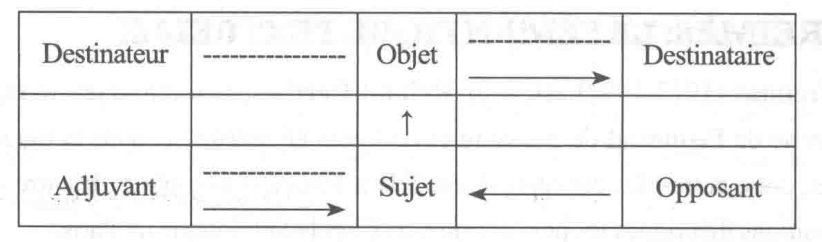
\includegraphics[width=.78\linewidth]{assets/ch11_actantiel_original.png}\end{center}

\subsubsection*{\textcircled{\scriptsize 2} Les trois axes}
Les actants sont situés par Greimas sur trois axes qui les relient de façon significative :
\begin{itemize}
\item L’axe du vouloir (sujet / objet). Le sujet est ce qui est orienté vers un objet. La relation établie entre le sujet et l’objet s’appelle « jonction ». Selon que l’objet est conjoint au sujet (par exemple, le prince veut la princesse) ou lui est disjoint (par exemple, un meurtrier réussit à se débarrasser du corps de sa victime), on parlera de « conjonction » ou de « disjonction ».
\item L’axe du pouvoir (adjuvant / opposant). L’adjuvant aide à la réalisation de la jonction souhaitée entre le sujet et l’objet, l’opposant y nuit. Par exemple, l’épée, le cheval, le courage, le sage aident le prince; la sorcière, le dragon, le château lointain, la peur lui nuisent.
\item L’axe du savoir (destinateur / destinataire). Le destinateur est ce qui demande que la jonction entre le sujet et l’objet soit établie. Par exemple, le roi demande au prince de sauver la princesse. Le destinataire est ce pour qui la quête est réalisée. En simplifiant, on peut dire que le destinataire bénéficiera de la réalisation de la jonction entre le sujet et l’objet. Par exemple, le roi, le royaume, la princesse, le prince, etc.
\end{itemize}

\subsection{L’isotopie}
Par isotopie, terme issu de la physique atomique, Julien Greimas désigne la répétition de sèmes (sèmes isotopants) dans un texte permettant de comprendre ce dernier. Dans \textit{Du sens} (1970), il en donne la définition suivante :
\origpage{335}{321}
\begin{quote}\small\itshape
Par isotopie, nous entendons un ensemble redondant de catégories sémantiques qui rend possible la lecture uniforme du récit, telle qu’elle résulte des lectures partielles des énoncés et de la résolution de leurs ambiguïtés qui est guidée par la recherche de la lecture unique.
\end{quote}
L’isotopie d’un texte peut donc être comprise comme le point commun sémantique entre toutes les phrases de ce texte qui en facilite la compréhension.

\subsubsection*{\textcircled{\scriptsize 1} La notion de molécule sémique}
Une molécule sémique est un ensemble d’au moins deux sèmes présents plusieurs fois dans une même unité sémantique. Quand une même molécule sémique est répétée, on a une isotopie. A la lecture de la plupart des poèmes en prose des \textit{Illuminations} de Rimbaud, des poèmes hermétiques de Mallarmé, ou des poèmes surréalistes de Paul Eluard, le lecteur non averti aura les plus grandes difficultés à comprendre la « logique » des phrases. Mais en repérant les molécules sémiques et leur répétition (c’est-à-dire les isotopie)\ednote{原文 les isotopie 应为 les isotopies。概念上，复现单个义素也可构成语义同位关系；“义素分子复现”不能取代全部 isotopie 的定义。本页首段与下文“曙光”例本身即按单个共同义素解释。} dans le poème, il pourra commencer à « comprendre le poème » grâce aux sèmes communs à plusieurs phrases sans liens apparents.

\subsubsection*{\textcircled{\scriptsize 2} Exemples en poésie}
Pour illustrer les notions d’isotopie et de molécule sémique, prenons deux exemples tirés de poèmes de Paul Éluard :

\noindent\textbf{Ex :} L’aube allume la source.

Assez peu compréhensible si l’on s’attache à une interprétation littérale, tout s’éclaire dès que l’on repère l’isotopie inchoative (du commencement), sème commun aux trois termes : aube, allumer et source. La même molécule fait l’objet de trois lexicalisations successives.

\noindent\textbf{Ex :} La terre est bleue comme une orange.

De prime d’abord,\ednote{此处惯用语为 De prime abord，原文混入了 d’abord 的 d’。} le lecteur sera choqué par l’absence de logique dans l’exemple ci-dessus : une orange n’est pas bleue. Pourtant, dès que l’on identifie l’isotopie de la rondeur (« terre », « orange ») et celle de la « couleur » (« bleue », « orange ») présentes simultanément dans le lexème « orange », alors encore une fois tout s’éclaire : l’isotopie rend le vers cohérent au niveau sémique. Ceci exemple\ednote{原文 Ceci exemple 应为 Cet exemple。} appelle deux remarques :
\begin{itemize}
\item d’une part, on voit qu’un même lexème peut participer à deux isotopies différentes : « orange » et « terre » participent toutes deux aux isotopies de la rondeur et de la couleur.
\item d’autre part, il est important de noter qu’une isotopie regroupe des sèmes communs, et non des lexèmes. Si c’est le cas, on parle alors de champ lexical.
\end{itemize}
Nous reviendrons sur l’isotopie un peu plus bas avec la sémantique interprétative de François Rastier. Dans l’immédiat, nous allons nous intéresser à un autre apport majeur de Greimas, le carré sémiotique.

\origpage{336}{322}
\subsection{Le carré sémiotique}
C’est dans le deuxième chapitre de sa \textit{Sémantique structurale} (1966), que Greimas présente son célèbre carré sémiotique développé avec \textbf{François Rastier}.

\subsubsection*{\textcircled{\scriptsize 1} Présentation}
Avec le modèle actantiel et l’isotopie, le carré sémiotique est une des théories les plus célèbres de l’École de Paris gravitant autour de Greimas. Modèle logico-sémantique, il permet de raffiner les analyses par oppositions en faisant passer le nombre de classes analytiques découlant d’une opposition de deux seulement chez Aristote (vie / mort) à quatre (vie / mort / vie et mort / ni vie ni mort), voire huit ou dix.\ednote{须区分基本项与复合项：下图四个基本位置是 A、B、非 B、非 A；“既 A 又 B”与“既非 A 又非 B”则是图中的第5、6个元项，并非与 A、B 并列的另两个基本角点。所谓“四类”与“四角”不能混为一谈。} Le carré sémiotique permet de faire apparaître et de visualiser :
\begin{itemize}
\item les relations de conjonction et de disjonction, placées respectivement au sommet et à la base du carré,
\item les relations de complémentarité (« deixis ») placées de chaque côté du carré. La deixis de gauche est positive, celle de droite négative.
\end{itemize}
\begin{center}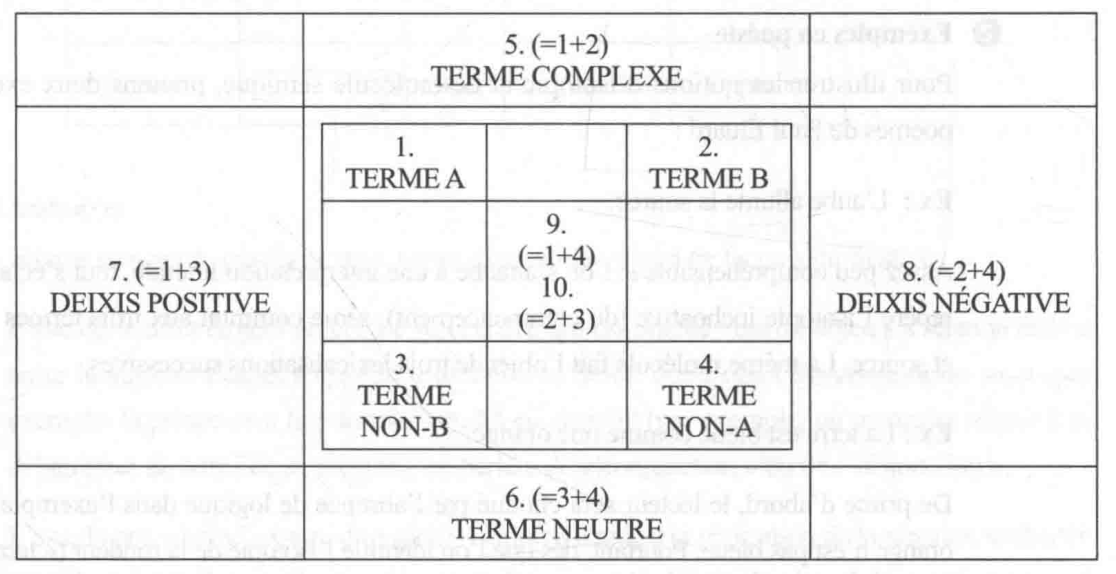
\includegraphics[width=.92\linewidth]{assets/ch11_square_extended_original.png}\end{center}

\subsubsection*{\textcircled{\scriptsize 2} Éléments constitutifs}
Le carré sémiotique est constitué des éléments suivants :
\begin{itemize}
\item des termes
\item des métatermes (termes composés)
\item un ou des objet (s) (classé (s) sur le carré)
\item un ou des sujet (s)-observateur (s)
\item le temps (de l’observation)
\end{itemize}
\minititle{1. Les termes}
Le carré sémiotique est constitué de quatre \textit{termes} situés au centre de carré) :\ednote{原文 au centre de carré) 多一右括号；通常可校为 au centre du carré。}
\origpage{337}{323}
\begin{itemize}
\item Position 1 (terme A)
\item Position 2 (terme B)
\item Position 3 (terme non-B)
\item Position 4 (terme non-A)
\end{itemize}
Les deux premiers termes forment l’opposition (relation de contrariété) à la base du carré. Par exemple, « vie » et « mort ». Les deux autres sont obtenus par la négation de chaque terme de cette opposition : « non vie » et « non mort ».

\minititle{2. Les métatermes}
Le carré sémiotique comporte six métatermes composés à partir des quatre termes et situés dans la partie extérieure du carré :
\begin{itemize}
\item Position 5 :\quad (terme 1 + terme 2)\quad terme complexe (conjonction)
\item Position 6 :\quad (terme 3 + terme 4)\quad terme neutre (disjonction)
\item Position 7 :\quad (terme 1 + terme 3)\quad déixis positive
\item Position 8 :\quad (terme 2 + terme 4)\quad déixis négative
\item Position 9 :\quad (terme 1 + terme 4)\quad pas de nom
\item Position 10 :\quad (terme 2 + terme 3)\quad pas de nom
\end{itemize}
Malgré leur nom, le terme « complexe » et le terme « neutre » sont des métatermes.\ednote{第6项按图为非 B 与非 A 的结合，即“既非 B 又非 A”。若将 disjonction 按形式逻辑“或”理解便会误读；该项应形式化为 $\neg B\land\neg A$，而不是 $\neg B\lor\neg A$。另，第9、10项在图中位于内部，与“均在外部”的说明不符。}

\subsubsection*{\textcircled{\scriptsize 3} Les relations de contrariété et de contradiction}
Le carré sémiotique, qui est donc une représentation visuelle de l’articulation logique d’une catégorie sémantique, offre un jeu de relations de complémentarité mais aussi de contrariété (s1/ s2) et de contradiction (s1 / non-s1; s2 / non-s2) représentées ci-dessous :
\begin{center}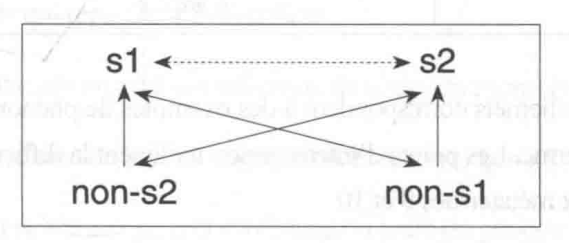
\includegraphics[width=.51\linewidth]{assets/ch11_square_relations_original.png}\end{center}
Regroupées sur le terme d’antonymie, les relations de contradiction et de contrariété se différencient de la manière suivante :
\begin{itemize}
\item Deux termes sont contradictoires lorsque l’affirmation de l’un équivaut à la négation de l’autre et réciproquement. Il n’y a pas de troisième position possible : par exemple, tout nombre est pair ou impair, sans autre position possible.\ednote{本例必须限定为整数。分数或无理数并不按整数奇偶性归为“偶数或奇数”；应为 tout nombre entier est pair ou impair。} C’est le principe du tiers exclu d’Aristote : soit une\origcont{338}{324} proposition est vraie, soit sa négation est vraie. Ainsi, dire qu’un nombre qu’il n’est pair\ednote{本句混杂两种结构且遗漏 pas；可校为 dire d’un nombre entier qu’il n’est pas pair，或 dire qu’un nombre entier n’est pas pair。} revient à dire qu’il est impair. En outre, la relation de contradiction est non gradable : un nombre n’est pas « plus ou moins » pair. Cette relation contradiction peut se marquer lexicalement (majeur/ mineur, mort/vivant), au moyen d’un préfixe (pair/impair), ou d’une particule négative (blanc/\textit{non}-blanc).
\item Deux termes sont contraires lorsque affirmer le premier revient à nier le second, mais nier le premier ne revient pas forcément affirmer le second.\ednote{原文 ne revient pas forcément affirmer 应补介词 à，即 ne revient pas forcément à affirmer。} Par exemple, dire qu’un objet est blanc signifie qu’il n’est pas noir, mais dire qu’il n’est pas blanc ne signifie pas qu’il est noir. En principe, les contraires ne peuvent être vrais ensemble, mais ils peuvent être faux ensemble : un objet peut, en effet, n’être ni noir ni blanc. Enfin, les contraires ne s’opposent pas comme deux termes d’une alternative exclusive : une troisième position est possible. Par exemple, le gris est ni noir ni blanc.\ednote{原文 le gris est ni noir ni blanc 应为 le gris n’est ni noir ni blanc。} Ils sont aussi gradables : un objet peut être plus ou moins chaud, plus ou moins blanc, plus ou moins grand, etc...
\end{itemize}
Tout ceci étant très théorique, je vous propose d’illustrer tout cela à l’aide d’un exemple de carré sémiotique.

\subsubsection*{\textcircled{\scriptsize 4} Application}
Le carré sémiotique ci-dessous illustre l’opposition entre masculin et féminin :
\begin{center}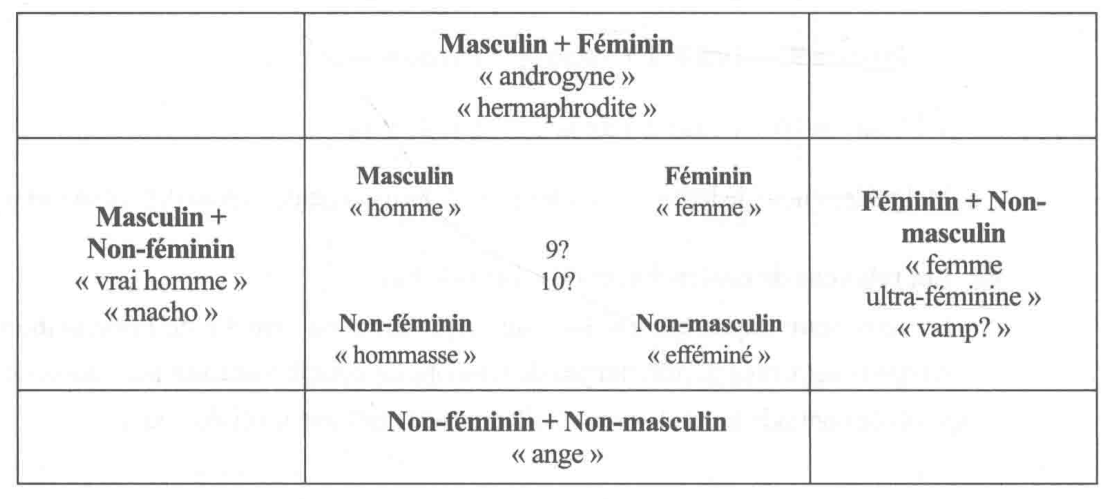
\includegraphics[width=.92\linewidth]{assets/ch11_square_gender_original.png}\end{center}
Les mots entre guillemets correspondent à des exemples de phénomènes classables dans un terme ou dans un métaterme. Les points d’interrogation indiquent la difficulté de trouver des phénomènes correspondant aux métatermes 9 et 10.\ednote{原图引号内的词是作者选择的文化联想例项，不应当作现实人物的性别分类定义。特别是图中“男性／女性”“男性化／女性化”并非同一对概念；将两者直接等同会使方阵的比较维度发生变化。本版保留原图及措辞。}

\subsubsection*{\textcircled{\scriptsize 5} Niveaux d’analyse}
Quelques remarques concernant l’exploitation et les niveaux d’analyse du carré sémiologique. Prenons pour exemple l’opposition entre « vie » et « mort ».
\begin{itemize}
\item Il convient d’abord de distinguer l’existence (ou non) dans le réel de ce que recouvre une position donnée. Par exemple, dans le réel, on ne peut être « mort » et « vivant » simultanément (position 5 : terme A + terme B). Mais c’est le cas dans la fiction, des vampires\origcont{339}{325} et des zombies.
\item Il convient ensuite de distinguer la possibilité (ou pas) de « lexicaliser » une position du carré, c’est-à-dire de la nommer par un mot ou une expression existant dans notre langue. Par exemple, le terme neutre « ni vie ni mort », c’est-à-dire la position 6 (non-B + non-A), qui pourrait désigner le chat de Schroedinger,\ednote{这里把 Schrödinger 的猫归为“既非生又非死”并不严谨。思想实验中的量子叠加不能等同于经典逻辑的两个否定项的合取；它不是方阵第6位的物理证明。参见第四章既有校勘及原论文译文\ecite{20}。} n’a pas de véritable lexicalisation en français. Par contre, « ni content ni triste » peut être lexicalisé par l’adjectif « indifférent ».
\item Enfin, notez que les métatermes 9 (terme A + terme non A) et 10 (terme B + terme non B), en plus de ne pas pouvoir être lexicalisés, ne sont pas non plus reconnus dans la sémiotique classique, cela afin de respecter le principe aristotélicien de non-contradiction qui interdit d’affirmer et nier le même terme ou la même proposition. Nous avons déjà rencontré ce principe dans le chapitre consacré à la logique, mais je pense qu’il n’est pas inutile de le rappeler ci-dessous :
\begin{quote}\small\itshape
Il est impossible qu’un même attribut appartienne et n’appartienne pas en même temps et sous le même rapport à une même chose.
\end{quote}
\end{itemize}
Pour terminer sur ce point, sachez que le carré sémiotique peut être utilisé comme outil d’analyse des discours textuels et visuels notamment dans le domaine du marketing, de la publicité et de la communication. À partir des années 1980, la sémiotique greimassienne a également été utilisée dans le champ des études de marchés, notamment à l’initiative des sémiologues \textbf{Jean-Marie Floch} et \textbf{Jean-Pierre Martinez}.

\section{FRANÇOIS RASTIER : LA SÉMANTIQUE INTERPRÉTATIVE}
Le sémanticien \textbf{François Rastier} (1945-), qui a étudié auprès de Greimas et de Pottier, est considéré comme le fondateur de la sémantique interprétative. Il s’agit d’une synthèse « de seconde génération » de la sémantique structurale européenne, développée à la suite des travaux de Bréal et de Saussure, puis de Hjelmslev, de Greimas, et de Pottier. Ses unités de base (entre autres, le sème et l’isotopie) ont été intégrées dans une théorie générale des formes sémantiques qui repose sur trois paliers :
\begin{itemize}
\item la microsémantique, rattachée aux paliers inférieurs du texte (du morphème au lexème)
\item la mésosémantique, rattachée aux paliers intermédiaires (du syntagme fonctionnel à la période)
\item la macrosémantique, rattachée aux paliers supérieurs du texte (la période et jusqu’au texte)
\end{itemize}
En simplifiant, on peut dire que ces trois paliers correspondent, respectivement, au mot, à la phrase et au texte.

\subsection{Les trois classes sémantiques}
En rapport avec les trois paliers, Rastier distingue trois classes sémantiques, que nous allons présenter par ordre de généralité décroissante. Précisons pour ce qui va suivre que pour Rastier, le sémème est le\origcont{340}{326} signifié d’un morphème.

\subsubsection*{\textcircled{\scriptsize 1} La dimension}
La dimension est la classe de plus grande généralité. Elle inclut des sémèmes ayant le même trait générique de plus grande généralité, appelé « sème macrogénérique ». Les dimensions sont regroupées par oppositions :

\noindent\textbf{Ex :} //animé// vs //inanimé//, //concret// vs //abstrait//, //humain// vs //animal//, //animal// vs //végétal//, etc.

\subsubsection*{\textcircled{\scriptsize 2} Le domaine}
Le domaine est une classe intermédiaire qui comprend des sémèmes (plus exactement des sous-ensembles de sémèmes) ayant un même trait générique de moindre généralité, appelé sème mésogénérique.

Par exemple, lorsque l’on consulte un dictionnaire, on y trouve des abréviations, comme \textit{cuis.} (pour cuisine), \textit{mar.} (pour maritime), \textit{jur.} (pour juridique), pour indexer la signification d’un terme. Ces indicateurs lexicographiques sont des domaines.

Rastier fait deux remarques intéressantes :
\begin{itemize}
\item d’une part, il observe qu’il n’existe pas de polysémie ni de relation métaphorique au sein d’un domaine donné. Le lexème « canapé », par exemple, est polysémique et renvoie soit au domaine //alimentation//, soit au domaine //habitation//.
\item d’autre part,, il remarque que la métaphore s’établit généralement entre domaines différents. Si par exemple un journal titre « l’ONU joue les arbitres dans le conflit syrien », la métaphore connecte deux domaines distincts : //sports// et //politique//.
\end{itemize}

\subsubsection*{\textcircled{\scriptsize 3} Le taxème}
Le taxème est la classe sémantique la plus basse : c’est à son niveau que se trouvent définis les sèmes de plus faible généralité (sèmes microgénériques) et les sèmes spécifiques. Par exemple, les sémèmes \{‘métro’, ‘train’, ‘autobus’, ‘autocar’\} relèvent du domaine //transports//, lui-même articulé en deux taxèmes :
\begin{itemize}
\item le taxème //ferré//, comprenant les sémèmes « métro » et « train », que l’on peut à leur tour opposer par les sèmes spécifiques /intra-urbain/ et /extra-urbain/
\item le taxème //routier//, comprenant les sémèmes « autobus » et « autocar », opposables eux aussi, par les sèmes spécifiques /intra-urbain/ et /extra-urbain/.
\end{itemize}
Prenons un exemple pour illustrer les notions de dimension, domaine et taxème.

\subsubsection*{\textcircled{\scriptsize 4} Application}
Le taxème des //couverts// (ustensiles) comporte trois sémèmes : fourchette, couteau, et cuillère.
\origpage{341}{327}
Chacun contient le sème microgénérique /couvert/, mais se distingue des autres sémèmes du même taxème avec un sème spécifique, comme suit :
\begin{itemize}
\item fourchette : /pour piquer/
\item couteau : /pour couper/
\item cuillère : /pour contenir/
\end{itemize}
Comme le taxème //couverts// est lui-même englobé dans le domaine //alimentation//, les trois sémèmes ci-dessus contiennent eux-aussi le sème mésogénérique //alimentation//. Par ailleurs, ces trois sémèmes participent également à une dimension commune : /concret/ et /inanimé/.

Par conséquent, si l’on prend comme exemple le sémème « cuillère », il contient les sèmes suivants :
\begin{itemize}
\item sème /couvert/ : microgénérique (appartenance à un taxème)
\item sème /alimentation/ : mésogénérique (appartenance à un domaine)
\item sème /concret/ et /inanimé/ : macrogénérique (appartenance à une dimension)
\item sème spécifique /pour contenir/, opposé aux autres sèmes spécifiques de « couteau » et de « fourchette »
\end{itemize}

\subsection{Typologie sémique}
Il ne faut maintenant apporter certaines précisions\ednote{原文 Il ne faut maintenant apporter 既不构成完整否定，也与即将补充说明的语境相反；可校为 Il faut maintenant apporter。} découlant du point précédent sur les classes de sèmes.

\subsubsection*{\textcircled{\scriptsize 1} Sèmes génériques et sèmes spécifiques}
Comme Pottier, Rastier effectue une distinction entre sèmes génériques et sèmes spécifiques. Selon sa typologie sémique :
\begin{itemize}
\item Le sème générique marque l’appartenance du sémème à une classe sémantique : il peut être microgénérique (relatif à un taxème), mésogénérique (relatif à un domaine), ou macrogénérique (relatif à une dimension).
\item Le sème spécifique, quant à lui, marque l’opposition du sémème à un ou plusieurs sémèmes de la classe à laquelle il appartient : on peut le rapprocher du sémantème de Pottier.
\end{itemize}
Ainsi, dans l’exemple ci-dessus, « couteau » et « cuiller », de par leur appartenance au même taxème //couvert//, ont le même sème microgénérique /couvert/ mais s’opposent par les sèmes spécifiques /pour couper/ vs /pour contenir/.

Prenons un autre exemple :
\begin{itemize}
\item Si la classe considérée est \{ « femme » vs « homme »\}, alors « femme » peut avoir pour sème
\origcont{342}{328} générique /personne/ et pour sème spécifique /de sexe féminin/.
\item Si la classe considérée est \{ « femme » ou « demoiselle »\}, alors aux sèmes génériques /personne/ et /de sexe féminin/, il faudra ajouter le sème spécifique /qui a été ou est mariée/.\ednote{此项只能描述特定传统称谓系统中 femme 与 demoiselle 的一种对比义，不能作为 femme 所有用法的必要义素；未婚女性仍可称 femme。本文强调 taxème 随比较集合而定，故例子的适用范围须同时保留。}
\end{itemize}

\subsubsection*{\textcircled{\scriptsize 2} Sèmes inhérents et sèmes afférents}
Pour Rastier, en plus d’être spécifiques ou génériques, les sèmes peuvent être inhérents ou afférents :
\begin{itemize}
\item Les sèmes inhérents sont les composants sémantiques invariants et fixés par la norme sociale du lexème. Rastier les définit comme l’extrémité d’une relation symétrique entre deux sémèmes appartenant au même taxème.
\item Les sèmes afférents sont définis par Rastier par comme\ednote{par Rastier par comme 中第二个 par 属衍字，应为 par Rastier comme。} les traits sémantiques dont l’actualisation résulte d’une contrainte contextuelle (à la différence des traits inhérents, qui sont hérités par défaut du type de l’occurrence).
\end{itemize}
Il introduit ainsi la distinction entre les sèmes inhérents dénotatifs, distinctifs, définitoires et universels, et les sèmes afférents connotatifs, non-distinctifs, non définitoires et non universels.\ednote{此处“universels”不能理解为超越所有语言、文化与语境的普遍必然性；紧接的解释仍将固有义素限定于语言的功能系统。附加义素也可来自共同社会规范，不必只是个人联想；二分并非与“有无解释作用”一一对应。参见本章下文对 classème、sémantème 及语境激活的讨论。} Pour lui, les sèmes inhérents relèvent du système fonctionnel de la langue, alors que les sèmes afférents relèvent d’autres types de codifications, comme les normes socialisées ou idiolectales. Puis il précise :
\begin{quote}\small\itshape
À la différence de la formulation inaugurale de Pottier, nous introduisons les sèmes afférents (« traits connotatifs » selon lui) dans le classème et dans le sémantème, au lieu de les regrouper dans une classe ad hoc (le virtuème).
\end{quote}
Il s’agit donc d’un problème de définition. En voici un autre : si pour Jacqueline Picoche le sémème est un ensemble de sèmes, à savoir de traits pertinents (ou distinctifs) sémantiques, le sémème pour François Rastier comprend des traits pertinents (sèmes inhérents) mais aussi des traits non pertinents (sèmes afférents).

\subsubsection*{\textcircled{\scriptsize 3} Application}
Après avoir présenté ces différences de définition, je vous propose d’illustrer tout cela par une petite application. Si l’on prend le titre de l’ouvrage de Stendhal \textit{Le Rouge et Le Noir}, on a :
\begin{itemize}
\item un taxème avec pour sème générique : /couleur/
\item les sèmes spécifiques : /rougeur/ vs /noirceur/
\end{itemize}
Par ailleurs, on sait que Julien hésite dans le choix de sa carrière entre l’église ou l’armée : nous avons donc :
\begin{itemize}
\item un taxème avec pour sème générique : /carrière/
\item les sèmes spécifiques : /église/ vs /armée/
\end{itemize}

\origpage{343}{329}
Ainsi :
\begin{itemize}
\item /couleur/ est un sème générique inhérent
\item /rougeur/ et/noirceur/ sont des sèmes spécifiques inhérents
\item /carrière/ est un sème générique afférent (on pourrait dire connotatif)
\item /armée/ et /église/ sont des sèmes spécifiques afférents
\end{itemize}
En approfondissant sa réflexion sur les sèmes afférents, Rastier a introduit les notions de sèmes actualisés et virtualisés.

\subsubsection*{\textcircled{\scriptsize 4} Sèmes actualisés et sèmes virtualisés}
Cette typologie s’inscrit dans une perspective de la sémantique textuelle, c’est-à-dire de l’étude des sémèmes en contexte. La définition initiale est gardée, mais Rastier note que les sèmes afférents n’ont de caractère définitoire au même titre que les sèmes inhérents.\ednote{否定缺少 pas，可校为 n’ont pas de caractère définitoire au même titre que les sèmes inhérents。按上文所述，附加义素仍能在具体文本中参与释义，不应把此句理解成“附加义素没有意义”。}

Prenons comme exemple le sémème « corbeau »: Rastier note que le sème /péjoratif/ n’est pas définitoire de « corbeau », mais qu’il peut être « actualisé » dans une expression comme « un corbeau de mauvais augure » : on dira alors que, du fait du contexte « de mauvais augure », il est actualisé dans « corbeau ».

Sur cette base, Rastier oppose les sèmes actualisés (activés par le contexte) et les sèmes virtualisés (neutralisés dans le contexte). Il donne comme exemple un extrait du roman \textit{Madeleine Férat} (1868) de Zola :

Ex : Guillaume était la femme dans le ménage, l’être faible qui obéit, qui subit les influences de la chair et de l’esprit.
\begin{itemize}
\item Dans ce contexte, le trait /faiblesse/, fortement récurrent (« faible », « obéit », « subit »), est actualisé. Il apparaît comme sème inhérent de « faible » et comme sème afférent de « femme ».
\item En revanche, le trait inhérent du sémème « femme », /sexe féminin/, est neutralisé parce que incompatible avec le trait /sexe masculin/ inhérent à Guillaume.
\end{itemize}
Vous aurez remarqué que le critère contextuel l’emporte donc sur celui qui relève du système fonctionnel de la langue. Il s’agit d’une étude dynamique du sens lexical.

\subsection{L’isotopie}
Déjà évoquée avec Julien Greimas, l’isotopie ne vous est pas étrangère. Rastier la définit ainsi :
\begin{quote}\small\itshape
On appelle isotopie toute itération d’une unité linguistique. L’isotopie élémentaire comprend donc deux unités de la manifestation linguistique. Cela dit, le nombre des unités constitutives d’une isotopie est théoriquement indéfini.
\end{quote}

\origpage{344}{330}
Rastier a introduit l’isotopie dans sa typologie sémique présentées plus haut.\ednote{présentées 应随单数阴性 typologie 配合为 présentée。} Ainsi, la distinction entre sèmes spécifiques et génériques lui permet de construire des isotopies génériques et des isotopies spécifiques, fondamentales pour l’interprétation textuelle.

\subsubsection*{\textcircled{\scriptsize 1} Les isotopies génériques}
Comme les sèmes génériques, les isotopies constituées par la récurrence de sèmes génériques (isotopies génériques) permettent souvent d’établir la thématique du texte, et se divisent en trois classes :
\begin{itemize}
\item La récurrence d’un sème macrogénérique indexant des sémèmes appartenant à une même dimension constitue une isotopie macrogénérique.

Ex : Le hérisson insectivore n’est pas de la même famille que le porc-épic.

Ici, les traits /animé/ et /animal/ sont présents dans à peu près tous les termes : cette récurrence constitue une isotopie macrogénérique.
\item La récurrence d’un sème mésogénérique indexant des sémèmes appartenant à un même domaine constitue une isotopie mésogénérique.

Ex : L’amiral ordonna de larguer les voiles.

Ici, le trait /navigation/ est présent dans « amiral » et « larguer les voiles » : cette récurrence constitue une isotopie mésogénérique.
\item La récurrence d’un sème microgénérique indexant des sémèmes appartenant au même taxème constitue une isotopie microgénérique.

Ex : Whisky, coca ou vin blanc ?

Vous pouvez noter ici la récurrence du trait /apéritif/.

Ex : Votre entrecôte, vous la voulez, saignante, à point, bien cuite ?

Notez la récurrence du trait /degré de cuisson/. Ces récurrences constituent des isotopies microgénériques.
\end{itemize}

\subsubsection*{\textcircled{\scriptsize 2} Les isotopies spécifiques}
Les isotopies spécifiques, comme leur nom l’indique, reposent sur des récurrences de sèmes spécifiques, lesquels ne marquent pas l’appartenance des sémèmes à des classes, mais au contraire les distinguent en leur sein.

\subsubsection*{\textcircled{\scriptsize 3} Connexions métaphoriques et allotopie}
Selon Rastier, deux types de connexions sont possibles entre sémèmes ou groupes de sémèmes :
\begin{itemize}
\item La connexion métaphorique, qui relie deux sémèmes présents dans la suite linguistique (dans une comparaison, par exemple).
\origpage{345}{331}
\item La connexion symbolique, par exemple, dans une métaphore \textit{in absentia} dont le terme comparé est absent.
\end{itemize}
Les isotopies spécifiques peuvent participer à des connexions métaphoriques.

Par exemple, Victor Hugo, dans « Booz endormi », parle d’une « faucille d’or » (« dans le champ des étoiles ») pour évoquer la lune. Notez que le trait spécifique /en forme de croissant/ constitue une isotopie commune entre « lune » et « faucille ». Mais les deux sémèmes ne relèvent pas du même domaine (ni a fortiori du même taxème) :
\begin{itemize}
\item « lune » a pour domaine //astronomie// et pour taxème //corps céleste //
\item « Faucille » a pour domaine //agriculture// et pour taxème //instruments agricoles//
\end{itemize}
Dans une connexion métaphorique, les deux sémèmes connectés doivent posséder au moins un sème (générique) incompatible : c’est la relation d’allotopie, introduite dans les années 70 par le Groupe {\BBSixGreek μ}, et définie comme le rapprochement de deux domaines hétérogènes. Prenons un exemple :

Ex : Cette femme est une fleur.

Ici, la connexion métaphorique repose sur les sèmes génériques incompatibles : /humain/ et /végétal/.

\subsubsection*{\textcircled{\scriptsize 4} La notion de poly-isotopie}
Dans le cas où, dans un texte, plusieurs isotopies se superposent, Rastier parle de poly-isotopie. Dans son essai \textit{Systématique des isotopies}, il écrit :
\begin{quote}\small\itshape
Un même texte peut évidemment manifeste plusieurs isotopies enchevêtrées.\ednote{引文中 peut 后应接不定式 manifester，而非 manifeste；引文按底本照录。}
\end{quote}
Malgré son titre, cet article est en effet pour l’essentiel un exemple de description d’un texte poly-isotopique : le sonnet \textit{Salut} de Mallarmé, reproduit dans les exercices à la page suivante. Rastier commence par distinguer deux isotopies sémiques : celle du banquet et celle de la navigation. Chacune de ces isotopies est manifestée par un certain nombre de sémèmes. Parmi ces sémèmes on peut distinguer deux catégories :
\begin{itemize}
\item Certains sémèmes sont lisibles simultanément sur les deux isotopies. C’est le cas pour le sémème « salut », qui constitue le titre du poème. Au niveau de la première isotopie, il signifie geste de courtoisie. Au niveau de la seconde, il signifie sauvetage\origfoot{6}{Comme dans l’expression « une planche de salut ».}. Les sémèmes de cette première catégorie sont, dans l’analyse du poème de Mallarmé, les plus nombreux.
\item D’autres sémèmes ne sont lisibles que sur une isotopie. Ainsi le sémème vers n’est lu que sur la première, le sémème solitude n’est lu que sur la seconde.\ednote{此处把 vers 只归入前文所列的第一条“宴饮”同位线，有可能混淆了随后练习要求辨认的其他同位线，或存在引文转述错位。vers 是底本可见字形，不擅自替换为同音的 verre；有待核对 Rastier 原文的分类表与解释，亦不在此代答练习。}
\end{itemize}

\origpage{346}{332}
Saurez-vous retrouver la troisième isotopie ? Rendez-vous tout de suite dans les exercices.

Notre prochain chapitre sera consacré au sixième (et dernier) domaine fondamental de la linguistique, à savoir à la pragmatique.

\Needspace{27\baselineskip}
\section*{Exercices}
\phantomsection\addcontentsline{toc}{section}{Exercices}
\noindent\textbf{I.\quad Complétez le tableau suivant avec les constituants du schéma actantiel :}
\par\smallskip
{\small\setlength{\tabcolsep}{6pt}\renewcommand{\arraystretch}{1.3}
\noindent\begin{tabularx}{\textwidth}{|p{.17\textwidth}|X|}\hline
\rule{0pt}{4em} & C’est le personnage qui doit accomplir une mission. Il s’agit généralement du personnage principal.\\\hline
\rule{0pt}{5em} & C’est ce que le sujet cherche à obtenir, l’enjeu ou l’objectif de sa quête. Il peut s’agir d’un objet réel (ex. un trésor) ou d’un élément abstrait (ex. l’amour).\\\hline
\rule{0pt}{5em} & C’est ce qui pousse le sujet à agir. Il apparaît donc au début de la mission. Le destinateur peut être un personnage, une chose, un sentiment, une idée, etc.\\\hline
\rule{0pt}{5.5em} & Ce sont tous ceux qui obtiennent un bénéfice, un avantage, à la fin de la mission. Le sujet peut être le destinataire, mais il est enrichi par l’obtention de l’objet de la quête.\\\hline
\rule{0pt}{4em} & Ce sont tous les personnages ou les éléments qui nuisent à la réalisation de la mission.\\\hline
\rule{0pt}{4em} & Ce sont tous les personnages ou les éléments qui aident le sujet à accomplir sa quête.\\\hline
\end{tabularx}}

\Needspace{9\baselineskip}
\origpage{347}{333}
\noindent\textbf{II.\quad Complétez le texte ci-dessous à l’aide des fonctions actantielles de Julien Greimas :}
\begin{keybox}
Paul (\rule{18mm}{.3pt}) demande à Marie (\rule{18mm}{.3pt}) d’user de son charme (\rule{18mm}{.3pt}) pour obtenir des informations (\rule{18mm}{.3pt}) cachées par le professeur (\rule{18mm}{.3pt}) sur l’examen de linguistique. Il (\rule{18mm}{.3pt}) pourra ensuite les revendre à fort prix aux étudiants (\rule{18mm}{.3pt}).
\end{keybox}

\Needspace{27\baselineskip}
\noindent\textbf{III.\quad Identifiez et analysez les trois isotopies dans ce sonnet de Stéphane Mallarmé (extrait de \textit{Poésies}, 1899) :}
\begin{center}
\textbf{SALUT}\par\medskip
Rien, cette écume, vierge vers\\
À ne désigner que la coupe;\\
Telle loin se noie une troupe\\
De sirènes mainte à l’envers.\par\medskip
Nous naviguons, ô mes divers\\
Amis, moi déjà sur la poupe\\
Vous l’avant fastueux qui coupe\\
Le flot de foudres et d’hivers;\par\medskip
Une ivresse belle m’engage\\
Sans craindre même son tangage\\
De porter debout ce salut\par\medskip
Solitude, récif, étoile\\
À n’importe ce qui valut\\
Le blanc souci de notre toile.
\end{center}

\Needspace{10\baselineskip}
\noindent\textbf{IV.\quad Effectuez l’analyse sémique des sémèmes suivants :}
\begin{keybox}
\begin{enumerate}[label=\arabic*.]
\item Un citron, une clémentine, une orange, un pamplemousse.
\item Des bottes, des pantoufles, des escarpins, des espadrilles, des sandales, des baskets.
\item Une conférence, un exposé, une harangue, une déclaration, un sermon, un éloge, un plaidoyer, un réquisitoire.
\end{enumerate}
\end{keybox}

\Needspace{9\baselineskip}
\noindent\textbf{V.\quad Quels sont les sèmes génériques et les sèmes spécifiques des sémèmes suivants ?}
\begin{keybox}
\begin{enumerate}[label=\arabic*.]
\item Un parapet, une rambarde, une glissière, un garde-fou, une barrière, une main-courante, un garde-corps.
\item Une voie, une chaussée, une rue, une route, un sentier, une allée, un chemin, une avenue, un boulevard, un cours, une bretelle, une voie express.
\end{enumerate}
\end{keybox}

\origpage{348}{334}
\section*{Pour aller plus loin}
\phantomsection\addcontentsline{toc}{section}{Pour aller plus loin}
\begin{flushleft}\small
\setlength{\parskip}{.5em}
COURTÉ (J.). \textit{Analyse sémiotique du discours : de l’énoncé à l’énonciation.} Paris, Hachette, 1991.\ednote{作者姓氏应作 Courtés，而非 Courté；本页与 Greimas 合著条中的 COURTÉ 同误。此处书目保留底本拼法，供检索时注意；书名及版本资料参见\ecite{55}。}

FLOCH (J.-M.) \textit{Quelques concepts fondamentaux en sémiotique générale.} Paris-Amsterdam, Éditions Hadès-Benjamins, 1985.

GREIMAS (A. J.). \textit{Du sens.} Paris, Seuil, 1970.

GREIMAS (A. J.). \textit{Du sens II.} Paris, Seuil, 1983.

GREIMAS (A. J.). \textit{Sémantique structurale}[1966]. Paris, P.U.F. 1986.

GREIMAS (A. J.) et COURTÉ (J.). \textit{Sémiotique : dictionnaire raisonné de la théorie du langage.} Paris, Hachette, 1993.

HJELMSLEV (Louis Trolle). \textit{Le langage.} Paris, Minuit, 1991.

HJELMSLEV (Louis Trolle). \textit{Prolégomènes à une théorie du langage.} Paris, Minuit, 1971.

JAKOBSON (R.). \textit{Linguistique et poétique}, dans \textit{Essais de linguistique générale.} Paris, Minuit, 1963.

MARTINET (André). \textit{Connotations, poésie et culture}, dans \textit{To Honor Roman Jakobson.} La Haye, Mouton, 1967, vol. II.

PROPP (Vladimir). \textit{Morphologie du conte.} Paris, Seuil, 1970.

RASTIER (François). \textit{L’isotopie sémantique, du mot au texte.} thèse de Doctorat d’État, Université de Paris-Sorbonne, 1985.

RASTIER (François). \textit{Sémantique et recherches cognitives.} Paris, P.U.F., 1991.

RASTIER (François). \textit{Sémantique interprétative.} Paris, P.U.F., 1987.
\end{flushleft}

\Needspace{27\baselineskip}
\section*{Glossaire}
\phantomsection\addcontentsline{toc}{section}{Glossaire}
\gloss{actant/analyse actantielle 主目，主语}{在生成语法里，与动词相关的某个名词的题元角色。\ednote{此词条把 actant、analyse actantielle 和题元角色混在一起，且“主目”疑为排印讹误，未据推测订字。本章的 actant 指行动元，analyse actantielle 指行动元分析；行动元不限于语法主语，也不与生成语法中的 theta-role 自动等同。见本章六行动元与三个轴的定义。}}
\origpage{349}{335}
\gloss{analyse sémique 语义分析}{关于意义的研究。\ednote{该释义过宽，更接近 sémantique。按本章第三节的定义，analyse sémique 特指把词义或义位分解为义素，并比较其共同与区别特征的“义素分析”。}}
\gloss{connotation 内涵意义}{词或短语的基本意义之外的意义。}
\gloss{dénotation 指示意义}{将词或短语同现实世界或虚构或可能世界里的现象联系起来的那部分意义。}
\gloss{glossématique 语符学}{指丹麦哥本哈根学派创立的语言学科。语符学集中研究语言的内在结构，力图用符号逻辑建立“语言的代数”，用一套形式定义来描写语言。}
\gloss{isotopie 同位素学}{具有相同核电荷数但质量数不同的原子互为同位素。\ednote{此处误用物理学同位素的释义来解释本章的语义学术语。语义学 isotopie 指文本中义素等意义特征的重复所形成的语义一致性／同位线，不是关于原子核或同位素的学科。原文物理学定义保留，但不能据此理解本章 Greimas、Rastier 的分析；参见本章 IV.2、V.3。}}
\gloss{sémantique 语义学；语义学的}{关于意义的研究。研究语言的意义有多种不同方法，如哲学家研究语言表达法之间的关系；语言学家研究语言的语义结构，并区分不同的意义种类。}
\gloss{sens}{在一种语言的词汇中，一个词或短语（即词位）与其他词语发生关系时所处的地位。}
